\chapter{Conceptos Generales}

\epigraph{\textit{''El único sistema verdaderamente seguro es aquel que se encuentra apagado, enterrado en un bloque de hormigón en una habitación sellada con plomo y vigilada por guardias armados. Incluso entonces tendría mis dudas''}}{--- Gene Spafford}

Tal y como Gene Spafford aseguraba con sus palabras \cite{gene-spafford}, la seguridad informática no es una ciencia infalible y el sistema verdaderamente seguro es una quimera, algo que no existe y a su vez resulta inalcanzable. Partiendo de ese punto, la seguridad informática tiene diversos objetivos que surgen de la necesidad de proteger la información y los sistemas informáticos cada vez más en auge. Objetivos como por ejemplo:
\begin{itemize}
	\item Minimizar y gestionar los riesgos y detectar los posibles problemas y amenazas de seguridad.
	\item Garantizar la utilización adecuada del sistema y la información.
	\item Limitar las pérdidas y conseguir a la adecuada recuperación del sistema en caso de un incidente de seguridad.
	\item Cumplir con el marco legal los requisitos impuestos por los clientes en sus contratos.
\end{itemize}

Existen numerosas definiciones para el término seguridad informática. En esencia, la seguridad informática es el área de la informática que se enfoca tanto en la protección de sistemas como en la protección de la propia información. 

Sin embargo, esa escueta definición resulta insuficiente y se hace necesario distinguir entre dos conceptos. Por una parte tenemos el concepto de seguridad informática y por otra parte el concepto de seguridad de la información. Aunque al principio ambos conceptos pueden parecer sinónimos, se tratan de áreas diferentes.

%------------------------------------------------------------------------------

\section{Seguridad Informática}

Existen un gran número de definiciones para el concepto de seguridad informática. Según INTECO (Instituto Nacional de Tecnologías de la Comunicación, ahora INCIBE), la seguridad informática consiste en \textit{la protección de las infraestructuras TIC que soportan un negocio o empresa} \cite{inteco-defs}. En la norma ISO 7498, en la que se recoge el modelo OSI (modelo de referencia creado en 1980 para arquitecturas de red, en contraposición a la heterogeneidad del modelo TCP/IP), se define la seguridad informática como \textit{una serie de mecanismos que minimizan la vulnerabilidad de bienes y recursos en una organización} \cite{iso-7498}.

Aunque existen numerosas definiciones para el concepto de seguridad informática, por lo general engloban el carácter de protección de cualquier tipo de recurso tecnológico informático, muchas veces supeditado a su uso en una organización, aunque no es necesariamente obligatorio.

%------------------------------------------------------------------------------

\section{Seguridad de la Información}

Ligado al concepto de seguridad informática se encuentra el concepto de seguridad de la información. Según INTECO, la seguridad de la información consiste en \textit{la protección de los activos de información fundamentales para el éxito de cualquier organización} \cite{inteco-defs}.

En una definición más antigua, elaborada en la norma ISO/IEC 17799 \cite{iso-17799} se define la seguridad de la información como \textit{la preservación de la CID}, acrónimo de “Confidencialidad, Integridad y Disponibilidad”. El concepto de CID es uno de los pilares de la seguridad de la información, en el que se ahondará más adelante.

Mientras que la seguridad informática se encarga de proteger las infraestructuras, es decir, se centra en un plano más técnico, la seguridad de la información no tiene porque hacer referencia a ningún tipo de tecnología informática o de comunicación. Los activos de información pueden ser digitales, como correos electrónicos, páginas web, imágenes, bases de datos, etc. pero no  tiene por que ser necesariamente así. También se pueden clasificar como activos de información documentos en papel, contratos, faxes, etcétera.

Al igual que ocurre con la seguridad informática, es habitual tratar el término de la seguridad de la información a nivel empresarial, cuando no está exclusivamente ligado a ese campo.

%------------------------------------------------------------------------------

\section{Servicios de la Seguridad de la Información}
La seguridad de la información proporciona una serie de servicios que tienen como objetivo proteger todo tipo de activos de información, ya sea de una organización o de un usuario particular. La suma y complementación de estos servicios es lo que permite esa protección de la información.

\subsection[CID]{Confidencialidad, Integridad y Disponibilidad}

Dentro de estos servicios, existe el acrónimo CID (\textit{Confidencialidad, Integridad, Disponibilidad}, en inglés CIA (\textit{Confidentiality, Integrity, Availability})). CID engloba los 3 servicios de la seguridad de la información existentes más importantes \cite{iso-27000}.

\begin{figure}[H]
	\centering
	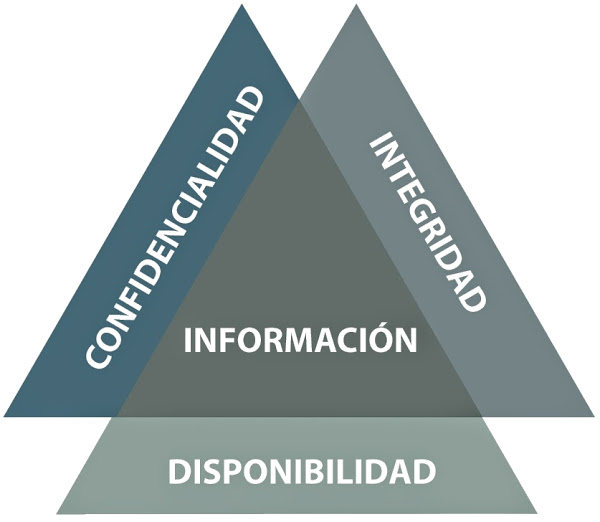
\includegraphics[width=200px]{cid}
	\caption{Confidencialidad, Integridad y Disponibilidad}
	\label{fig:cid}
\end{figure}

\begin{itemize}
	\item \textbf{Confidencialidad:} garantiza que la información no se ponga a disposición ni revela a individuos, entidades o procesos no autorizados.
	\item \textbf{Integridad:} garantiza que la información no se modifique malintencionadamente, por parte de individuos o procesos, durante su procesado o su transmisión, y en caso de modificarse, permite detectar dichas modificaciones.
	\item \textbf{Disponibilidad:} garantiza el acceso y utilización de la información y los sistemas de tratamiento de la misma por parte de los individuos, entidades o procesos autorizados cuando lo requieran. Además garantiza la recuperación de la información y de los sistemas de información en caso de posibles incidentes.
\end{itemize}

\subsection{Otros servicios}

Además de CID, existen otros servicios que complementan el concepto de seguridad informática. Aunque CID consiste en tres servicios que son de obligado cumplimiento para garantizar la seguridad de la información, no resultan suficientes, ya que no cubren todo tipo de casos en los que se puede comprometer la información. Entre el diverso número que existen, seguidamente se enumeran y definen algunos de ellos, considerados de los más relevantes \cite{apuntes-isma}.

\begin{itemize}
	\item \textbf{Autenticación:} garantiza que la identidad del creador de un mensaje es legítima. Permite asegurar la autoría de la información creada o modificada.
	\item \textbf{No repudio:} permite, mediante diferentes mecanismos, demostrar la autoría de un mensaje e impide que el usuario niegue esa circunstancia.
	\item \textbf{Autorización:} permite controlar el acceso a cierto sistema o información por parte de un usuario, permitiendo dicho acceso sólo a ciertos usuarios previamente designados, una vez superado el servicio de autenticación. 
	\item \textbf{Auditabilidad:} permite registrar y monitorizar la utilización de los distintos recursos del sistema por parte de los usuarios para garantizar el correcto uso del sistema y de su información.
	\item \textbf{Anonimato:} permite garantizar el anonimato de los usuarios que acceden a los recursos y consumen determinados tipos de servicios, preservando así su privacidad. Puede entrar en conflicto con otros ya mencionados, como la autenticación o la auditoría del acceso a los recursos.
	\item \textbf{Protección a la réplica:} impide que se haga uso de ataques de repetición que engañen al sistema provocando operaciones y modificaciones de la información no deseadas.
\end{itemize}
